\chapter{Attacchi TCP/IP}

\section{Livello di trasporto}
La responsabilità principale del livello di trasporto è la consegna 
dei dati da processo a processo. I singoli processi in esecuzione su un 
dato host sono identificati dai loro numeri di porta.

\begin{figure}[H]
    \centering
    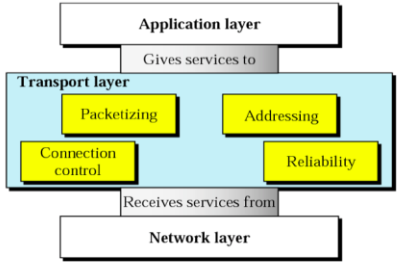
\includegraphics[width=0.7\linewidth]{chapters/8/images/trasporto.png}
\end{figure}

\noindent I due protocolli del livello di trasporto utilizzati in internet 
sono TCP e UDP.

\subsection{Porte}
Un numero di porta è un intero a 16 bit che assume un valore comprso 
tra 0 e 65535. I numeri di porta tra 0 e 1023 (i cosidetti \textit{numeri di
porta noti}) sono riservati ad applicazioni come HTTP, \dots

\section{TCP (Transmission Control Protocol)}
\begin{itemize}
    \item \textbf{Mittente:} suddivide i dati in pacchetti; ad ogni pacchetto è associato un numero di sequenza
    \item \textbf{Ricevitore:} riassembla i pacchetti nell'ordine corretto; i pacchetti persi vengono rispediti
\end{itemize}

\begin{figure}[H]
    \centering
    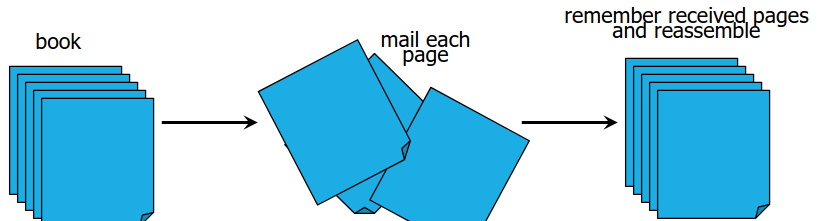
\includegraphics[width=1\linewidth]{chapters/8/images/tcp.png}
\end{figure}

\subsection{Flag TCP}
\begin{itemize}
    \item \textbf{SYN:} richiesta di connessione, primo pacchetto della comunicazione 
    \item \textbf{FIN:} intenzione del mittente di terminare la sessione
    \item \textbf{ACK:} conferma del pacchetto precedente
    \item \textbf{RST:} reset della sessione 
    \item \textbf{URG:} dati urgenti che vengono inviati con precedenza sugli altri (es. CTRL+C) 
\end{itemize}

\subsection{TCP handshake}
Le connessioni TCP vengono stabilite tramite un handshake a tre vie:
\begin{itemize}
    \item il server ha generalmente un listener passivo, in attesa di una richiesta di connessione 
    \item il client richiede una connessione inviando un pacchetto SYN 
    \item il server risponde inviando un pacchetto SYN/ACK, indicando un riconoscimento per la connessione 
    \item il client risponde inviando un ACK al server, stabilendo così la connessione
\end{itemize}

\begin{figure}[H]
    \centering
    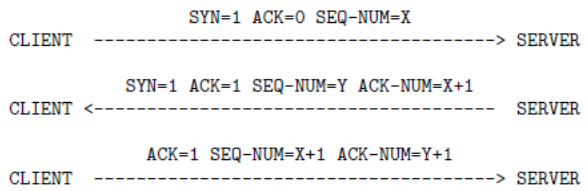
\includegraphics[width=0.8\linewidth]{chapters/8/images/tcp-handshake.png}
\end{figure}

\subsection{Problemi intrinsechi}
\begin{itemize}
    \item \textbf{Non c'è autenticazione} fra le parti; un utente malevolo potrebbe 
    intromettersi nella connessione fintanto che usa un \textit{sequence number} corretto 
    e gli indirizzi IP sono corretti 
    \item i \textbf{controlli di integrità} sono banali
\end{itemize}

\section{Spoofing}

\subsection{TCP spoofing}
Ogni connessione TCP ha uno stato associato:
\begin{itemize}
    \item numero di sequenza 
    \item numero di porta 
\end{itemize}

$\rightarrow$ è facile da indovinare, dato che si usano numeri di porta standard e numeri 
di sequenza prevedibili

\noindent È dunque possibile iniettare pacchetti in connessioni esistenti:
\begin{itemize}
    \item se l'attaccante conosce il numero di sequenza iniziale e la quantità di traffico, può indovinare 
    il probabile numero corrente 
    \item altrimenti, dato che la maggior parte dei sistemi accetta grandi finestre di numeri di sequenza per gestire 
    le perdite di pacchetti, invia un flusso di pacchetti con probabili numeri di sequenza
\end{itemize}

\subsection{IP spoofing}
Le autenticazioni locali su indirizzi IP sono insicure, specialmente 
all'interno di rete locali; l'header IP è falsificabile senza particolari 
difficoltà.
\begin{itemize}
    \item \textbf{Blind spoofing}
    
    \noindent Attacca da qualsiasi fonte; cerca di impersonare un host qualunque
    di internet, non facente parte della sottorete in cui si trova.
    
    \noindent \textit{Blind} perché l'attaccante non ha nessuna possibilità di vedere i 
    pacchetti mandati in risposta ai pacchetti \textit{"spoofati"} che ha spedito;
    questi ultimi saranno infatti spediti al vero host che l'attaccante sta impersonando, 
    impedendogli quindi di venire a conoscenza di \textit{ack number} e \textit{sequence number}
    corretti per continuare la connessione.

    \item \textbf{Non-blind spoofing}
    
    \noindent L'attaccante si trova nella stessa rete della vittima, quindi sarà in grado 
    di intercettare i pacchetti in risposta a quelli fraudolenti che ha inviato (tramite sniffer), e quindi 
    di ottenere il sequence number corretto.
\end{itemize}

\noindent I passaggi di IP spoofing sono:
\begin{enumerate}
    \item viene \textbf{scelta una vittima} e cercato un host considerato come fidato dalla vittima 
    \item si \textbf{disabilita l'host fidato} (ad esempio tramite SYN flooding)
    \item a questo punto si \textbf{contatta la vittima} e si ottiene un numero di sequenza valido, per provare 
    a predire il prossimo numero di sequenza 
    \item l'attaccante manda un pacchetto SYN utilizzando come IP mittente quello della macchina fidata. Anche se 
    l'hacker non riceve il SYN/ACK, può sempre rispondere in modo che la vittima pensi di aver stabilito correttamente la 
    connessione 
\end{enumerate}

\noindent La disabilitazione dell'host fidato è parte fondamentale, in quanto alla ricezione 
del pacchetto SYN/ACK potrebbe interrompere la connessione tramite un pacchetto RST.


\section{TCP session hijacking}

L'obiettivo è aprire una connessione con il server \textbf{impersonando la vittima}; 

\begin{itemize}
    \item L'attaccante apre una connessione autentica con il suo bersaglio (B), ricevendo un numero di sequenza 
    \item L'attaccante (C) si spaccia per il client (A)
    \begin{itemize}
        \item invia un pacchetto con l'indirizzo del client (A) nel campo dell'indirizzo sorgente
        e un numero di sequenza coerente con ciò che B si aspetta
    \end{itemize}
    \item Se l'attaccante indovina il numero di sequenza, il server presume di avere una connessione con A 
    \begin{itemize}
        \item L'attaccante non può vedere l'output di questa sessione, ma potrebbe eseguire comandi con i privilegi 
        di A sul server
    \end{itemize}
\end{itemize}

\begin{figure}[H]
    \centering
    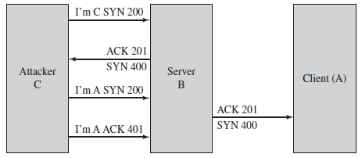
\includegraphics[width=0.8\linewidth]{chapters/8/images/tcp-hijack.png}
\end{figure}


\section{ACK storm}
Gli attacchi ACK storm si basano sul fatto che, quando si riceve un pacchetto con ACK più 
grande di quello inviato dal client ricevente, il client deve inviare l'ultimo pacchetto 
inviato all'altro lato e scartare il pacchetto ricevuto.

\noindent L'attacco prevede di:
\begin{itemize}
    \item prelevare un pacchetto da una connessione TCP tra un client e un server 
    \item generare due pacchetti, ciascuno inviato a una parte con l'indirizzo IP dell'altra
    \item inviare i pacchetti contemporaneamente
\end{itemize}

$\rightarrow$ la connessione entra in un ciclo infinito di ACK.

\noindent Come contromisura a questo attacco, si è modificato il protocollo facendo in modo che 
il pacchetto viene scartato senza dover rimandare la risposta.

\section{Attacco DoS}
Lo scopo è quello di impedire alla vittima di rispondere alle richieste; esistono 
due tipi di DoS:
\begin{itemize}
    \item \textbf{DoS bug:} sfrutta difetti di progettazione della vittima 
    \item \textbf{DoS flood:} vengono sfruttate delle bot-net per inondare di richieste la vittima
    \begin{itemize}
        \item un modo è quello di usare \textbf{ACK reflection attack:}
        
        \noindent L'attaccante invia del traffico con l'indirizzo IP della vittima ad un server intermedio (detto \textit{reflector}),
        che si occuperà di mandare le risposte alla vittima 

        $\rightarrow$ si può mandare una serie di SYN al reflector che inonderà la vittima di 
        SYN/ACK; la vittima vedrà l'IP del reflector e non quello dell'attaccante
    \end{itemize}
\end{itemize}

\subsection{SYN flood}
Prevede che l'attaccante \textbf{continui ad inviare richieste SYN al server} senza poi 
rispondere ai SYN/ACK ricevuti in risposta; in questo modo, il server dovrà dedicare risorse per rispondere 
ed attendere inutilmente che le connessione TCP aperte terminino l'handshake. L'idea è quella
di impedire al server di poter rispondere ad ulteriori richieste di connessione legittime.

\subsection{Contromisure ad attacco DoS}
Ci sono quattro approcci principali:
\begin{itemize}
    \item \textbf{aumentare le dimensioni del \textit{backlog}} (coda in cui il server memorizza le connessioni 
    iniziate che non hanno ancora terminato l'handshake)
    \item ridurre il \textbf{SYN-Received timer}, ovvero il tempo per cui una connesisone rimane nel backlog prima 
    che venga scartata 
    \item \textbf{SYN cookies:} il server inserisce le informazioni che di norma si salverebbero nel backlog 
    all'interno di un cookie che viene inserito nella risposta SYN/ACK inviata al client. Solo nel 
    momento in cui in server riceve risposta allora aprirà la connessione e le dedicherà risorse.

    \noindent Il cookie deve essere firmato e non modificabile; viene calcolato nel seguente modo 
    \begin{itemize}
        \item i primi \textbf{5 bit} sono dati da $t mod 32$, con $t$ \textbf{timestamp}
        \item i seguenti \textbf{3 bit} sono la codifica del numero di entry che il server avrebbe salvato nel backlog 
        \item gli ultimi \textbf{24 bit} sono il risultato di una funzione di hash, che prende in input:
        \begin{itemize}
            \item input IP server
            \item IP client
            \item porta del server
            \item porta client
            \item timestamp
        \end{itemize}
    \end{itemize}

    \noindent Nel momento in cui il client manda l'ACK in risposta con allegato il cookie, la \textbf{verifica}
        ha i seguenti passi:
        \begin{enumerate}
            \item viene verificato il timestamp per vedere se il pacchetto sia ancora valido 
            \item vien ricomputata la funzione di hash per vedere se il SYN sia ancora valido 
            \item vengono decodificati i 3 bit corrispondenti alla entry della coda di backlog
        \end{enumerate}
    \item \textbf{cancellazione di una entry a caso} per far posto a una nuova 
    \item uso di un \textbf{prolexic proxy:} si mette un proxy tra server e client; sarà il proxy a gestire 
    l'handshake, ed inoltrerà al server solo le richieste SYN di cui si riceve anche un ACK
\end{itemize}

\section{UDP (User Datagram Protocol)}
UDP è un protocollo di trasporto minimale che si limita ad inviare le informazioni sulla 
rete senza preoccuparsi che queste arrivino effettivamente a destinazione; non c'è nessun 
controllo del flusso e nessun riconoscimento.

\noindent Viene usato ad esempio per applicazioni di streaming.

\subsection{DDoS - NTP amplification}
Il protocollo NTP è usato per sincronizzare i \textit{clock} tra macchine diverse tramite UDP.

\noindent L'attacco consiste nello sfruttare il comando \texttt{monlist}, abilitato di default 
nelle vecchie versioni del protocollo, che permette di ottenere gli ultimi 600 IP che hanno fatto 
domanda al server NTP; successivamente si inonda di traffico UDP la vittima facendo IP spoofing.

\noindent \textit{Passaggi:}
\begin{itemize}
    \item L'attaccante usa una botnet per inviare pacchetti UDP con IP mittente della vittima 
    al server NTP, con i quali richiede l'esecuzione del comando \texttt{monlist}
    \item ogni pacchetto effettua una richiesta al server NTP che risponde all'IP della vittima 
    \item la rete della vittima viene inondata di traffico, circa 20 volte superiore a quello 
    delle richieste inviate dall'attaccante (la richiesta del comando \texttt{monlist} è circa 200 
    volte più piccola dell'output del comando stesso)
\end{itemize}

\noindent L'attacco viene definito di \textit{amplificazione} perché da una banda piuttosto piccola 
è possibile ricavare grosse quantità di dati con cui effettuare un DDoS tramite la \textit{reflection}
del server NTP.

\newpage
\section{ICMP (Internet Control Message Protocol)}
È un protocollo che permette la comunicazione tra host e router, per scambiare informazioni 
relative allo stato della rete (host irraggiungibili, echo delle richieste/risposte \dots).

\begin{figure}[H]
    \centering
    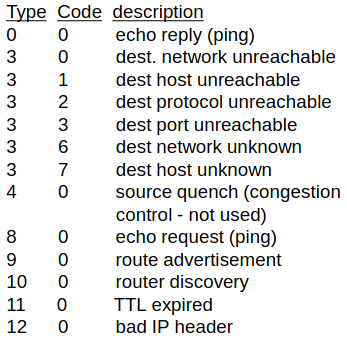
\includegraphics[width=0.6\linewidth]{chapters/8/images/icmp.png}
\end{figure}


\subsection{Attacco \textit{smurf} DDoS}

L'attacco prevede l'utilizzo di una \textbf{richiesta ICMP echo} (ping) e l'\textbf{IP spoofing}
per inviare alla vittima una quantità di dati di risposte echo che rendono inservibili 
altre richieste.

\noindent \textit{Passaggi:}
\begin{itemize}
    \item l'attaccante usa come mittente in una richiesta ICMP echo l'IP della vittima all'indirizzo
    di broadcast della rete 

    $\rightarrow$ la richiesta viene inoltrata a tutti gli host della rete 

    \item tutti gli host rispondono all'IP della vittima, causando il DDoS
\end{itemize}

\noindent La \textbf{contromisura} può essere scartare tutti i pacchetti che hanno come 
destinazione l'indirizzo di broadcast.

\newpage
\section{IP}
I datagrammi IP sono composti da diverse sezioni:
\begin{figure}[H]
    \centering
    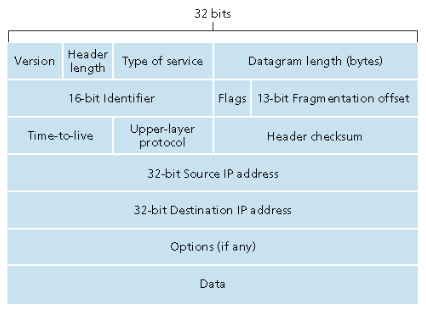
\includegraphics[width=0.8\linewidth]{chapters/8/images/ip.png}
\end{figure}

\noindent Durante il trasporto dei datagrammi IP è possibile che sia richiesta la loro frammentazione, 
per poi ricomporli lato ricevente.

\subsection{Teardrop attack}

In questo attacco, l'attaccante invia una serie di pacchetti che \textbf{vengono 
frammentati, ma non possono essere ricostruiti:} si inviano frame che dicono di avere 
posizioni di partenza e lunghezze in byte che si sovrappongono tra loro; come ad esempio:
\begin{itemize}
    \item \textit{posizione 0 e lunghezza 60 btye}
    \item \textit{posizione 30 e lunghezza 90 btye}
    \item \textit{posizione 40 e lunghezza 120 btye}
\end{itemize}

\noindent In questo caso viene sollevato un errore che manda in crash il sistema opeativo 
del server (DoS).

\noindent La \textbf{contromisura} consiste nello scartare tutti i frame che si riferiscono 
a pacchetti IP che risultano malformati.

\newpage
\subsection{Ping of Death}
Quando si usa il comando \textit{ping} di ICMP, bisogna rispettare una dimensione massima 
di $2^16$, ovvero la dimensione massima di un pacchetto.

\noindent L'attaccante può mandare un insieme di frame riferiti ad un pacchetto IP, la 
cui ricomposizione supera il limite imposto; in questo caso si verificherà un buffer overflow
che manderà in crash il sistema operativo.

\noindent Come nel caso precedente, la \textbf{contromisura} consiste nel controllare 
i frame e scartare quelli non validi.

\section{DNS amplification DDoS}
L'attacco consiste nell'\textbf{inviare una query DNS con IP mittente spoofato}, in 
modo che il DNS resolver risponda alla vittima. Il DoS è dato dal fatto che è possibile 
ricavare una query DNS che generi una risposta fino a 50 volte maggiore

$\rightarrow$ la vittima non è in grado di gestire il traffico della risposta (DoS)

\noindent Come in tutti gli attacchi di \textit{amplificazione}, la banda richiesta 
dall'attaccante è molto inferiore a quella con cui viene travolta la vittima.


